\documentclass[12pt]{article}
%\usepackage[T5,T1]{fontenc}
\usepackage{amssymb,amsmath}
%\usepackage{txfonts}
%\usepackage{fouriernc}
%\usepackage{ccfonts}
%\usepackage[varg]{txfonts}
%\usepackage{mathptmx}
%\usepackage{pxfonts}
%\usepackage{mathpazo}
%\usepackage{mathpple}
%\usepackage[charter]{mathdesign}
%\usepackage[utopia]{mathdesign}
%\usepackage{fourier}

%% Sanserif fonts
%\usepackage{arev}

%\usepackage{alltt} %%%%%%%%%%%%%%%%%%%%%%%%%%%% Use math in verbatim mode

%\usepackage{graphicx}
\usepackage{pdfpages}

%\usepackage{rotating}
\usepackage{framed}
% This lets you box text: e.g.
% \begin{framed}
% Put your text here. It'll appear in a box.
% \end{framed}

%\usepackage{fullpage} % smaller margins.
\frenchspacing % Shortens space between 2 sentences.
\setlength{\parindent}{0pt} % No par indent
\setlength{\parskip}{2ex} % 2 lines between pars.
\linespread{1.0} % Single-spaced. Change to 2.0 for double space, etc.

% This command lets you define new math operators:
\DeclareMathOperator{\stab}{stab}

% Eg for defining TeX functions:
%\newcommand{\mnom}[2]{\left(\negthickspace\binom{#1}{#2}\negthickspace\right)}% This one's used to denote ((n ; k)) := (n+k-1 ; k) = the number of ways to put k identical balls into n distinct boxes = the number of k-multisets on an n-set.

\renewcommand{\bf}{\bfseries}

%%%%%%%%%%% SYMBOLS %%%%%%%%%%%%%%%
\newcommand{\R}{{\bf R}}
\newcommand{\Q}{{\bf Q}}
\newcommand{\Z}{{\bf Z}}
\newcommand{\N}{{\bf N}}
\newcommand{\C}{{\bf C}}
\newcommand{\e}{\epsilon}
\newcommand{\f}{\phi}
\newcommand{\s}{\sigma}
\renewcommand{\r}{\rho}
%\newcommand{\G}{\Gamma}
\newcommand{\q}{\quad}
\newcommand{\nsub}{\trianglelefteq}
\newcommand{\<}{\langle}
\renewcommand{\>}{\rangle}
\newcommand{\inv}{^{-1}}

%%%%%%%%%%%%%%% DOCUMENT-SPECIFIC COMMANDS
\newcommand{\Customer}{C}
\newcommand{\Card}{K} 
\newcommand{\Order}{O}
\newcommand{\Item}{I}
\newcommand{\OrderItem}{U}
\newcommand{\Rating}{R}
\newcommand{\CID}{\text{CID}}
\newcommand{\IID}{\text{IID}}
\newcommand{\OID}{\text{OID}}
\newcommand{\email}{\text{email}}
\newcommand{\name}{\text{name}}
\newcommand{\phone}{\text{phone}}
\newcommand{\address}{\text{address}}
\newcommand{\cI}{\text{cI}}
\newcommand{\cN}{\text{cN}}
\newcommand{\expiry}{\text{expiry}}
\newcommand{\n}{\text{number}}
\newcommand{\category}{\text{category}}
\newcommand{\IIDi}{\text{IID1}}
\newcommand{\IIDii}{\text{IID2}}
\newcommand{\quantity}{\text{quantity}}
\newcommand{\price}{\text{price}}
\newcommand{\timestamp}{\text{timestamp}}
\newcommand{\ti}{\text{t1}}
\newcommand{\tii}{\text{t2}}

\newcommand{\HRule}{\rule{\linewidth}{0.5mm}}

%% This one lets you rotate a symbol:
%\newcommand{\GG}{\begin{sideways}\begin{sideways}$\G$\end{sideways}\end{sideways}}

%\nmid = does not divide

%%% Physics %%%
%\newcommand{\Favg}{\F_\text{avg}}
%\newcommand{\Fnet}{\F_\text{net}}

%\usepackage{color}
%\pagecolor{black}
%{\color{white}
\begin{document}
%\title{CSC343 A1}
%\author{Trong Truong \& Ross Gatih\\
%		\ \ \ 995 94 222 6 \ \ \ \  997 92 311 8}
%\date{Thursday 11 October 2012}
%\maketitle
%\tableofcontents

%\begin{titlepage}
	\begin{center}
	
	% Upper part of the page
	%\includegraphics[width=0.15\textwidth]{./logo}\\[1cm]    
	
	\textsc{\LARGE CSC343 A3}\\[1.0cm]
	
	%\textsc{\Large Final year project}\\[0.5cm]
		
	% Title
	%\HRule \\[0.4cm]
	{\huge \bfseries ER MODELLING AND \\ \vspace{6pt} DATABASE DESIGN}\\[1.0cm]
	%\HRule \\[1.5cm]
	
	%\vfill
	
	% Author and supervisor
	\begin{minipage}{0.4\textwidth}
	\begin{flushright} \large
	Ross Gatih\\
	997 92 311 8
	\end{flushright}
	\end{minipage}\hspace{24pt}
	\begin{minipage}{0.4\textwidth}
	\begin{flushleft} \large
	Trong Truong\\
	995 94 222 6
	\end{flushleft}
	\end{minipage}\\[1cm]
	
	%\vfill
	
	% Bottom of the page
	{\large Sunday 18 November 2012}
	
	\end{center}
%\end{titlepage}

\tableofcontents

\part{Assumptions}

\section{Setup and login phase}

{\bf Number of reviewers.} Each conference has a fixed number of reviewers assigned per paper.

{\bf Conference participant multiplicity.} Every user can participate in at most one role per conference, otherwise we have a conflict of interest. (E.g. a chair has the power to choose who gets to review a paper, so she might choose herself.)

{\bf Conference topic multiplicity.} Every conference can define its own topics, or use existing topics from other conferences.

{\bf File storage.} We'll only store filenames of papers, forms, and letters in the database. The files themselves will be stored on a hard drive somewhere outside the database.

\section{Submission phase}

{\bf Author conferencce participation.} An author may have an account without being registered in any conference. She may upload a paper without submitting it to any one.

{\bf Different submissions are different papers.} An author has the option to update an existing submission instead of submitting an identical copy, but that's application, not database-level design, so we don't have to worry about that.

{\bf Author VS coauthor.} We don't distinguish between authors and coauthors: everyone author of a paper is a coauthor.

\section{Reviewing phase}

{\bf Reviewer preference: bidding process.} To bid on a paper, a reviewer expresses her level of interest by assigning an integer between 0 (low) and 5 (high). 

{\bf Reviewer's choice.} A reviewer casts a vote of YES or NO on whether or not she thinks the paper should be published.

\section{Decision and publishing phase}

{\bf One letter per paper.} The chair sends only one acceptance notification letter per paper, to the coauthor who submitted it.

\part{ER diagram}

%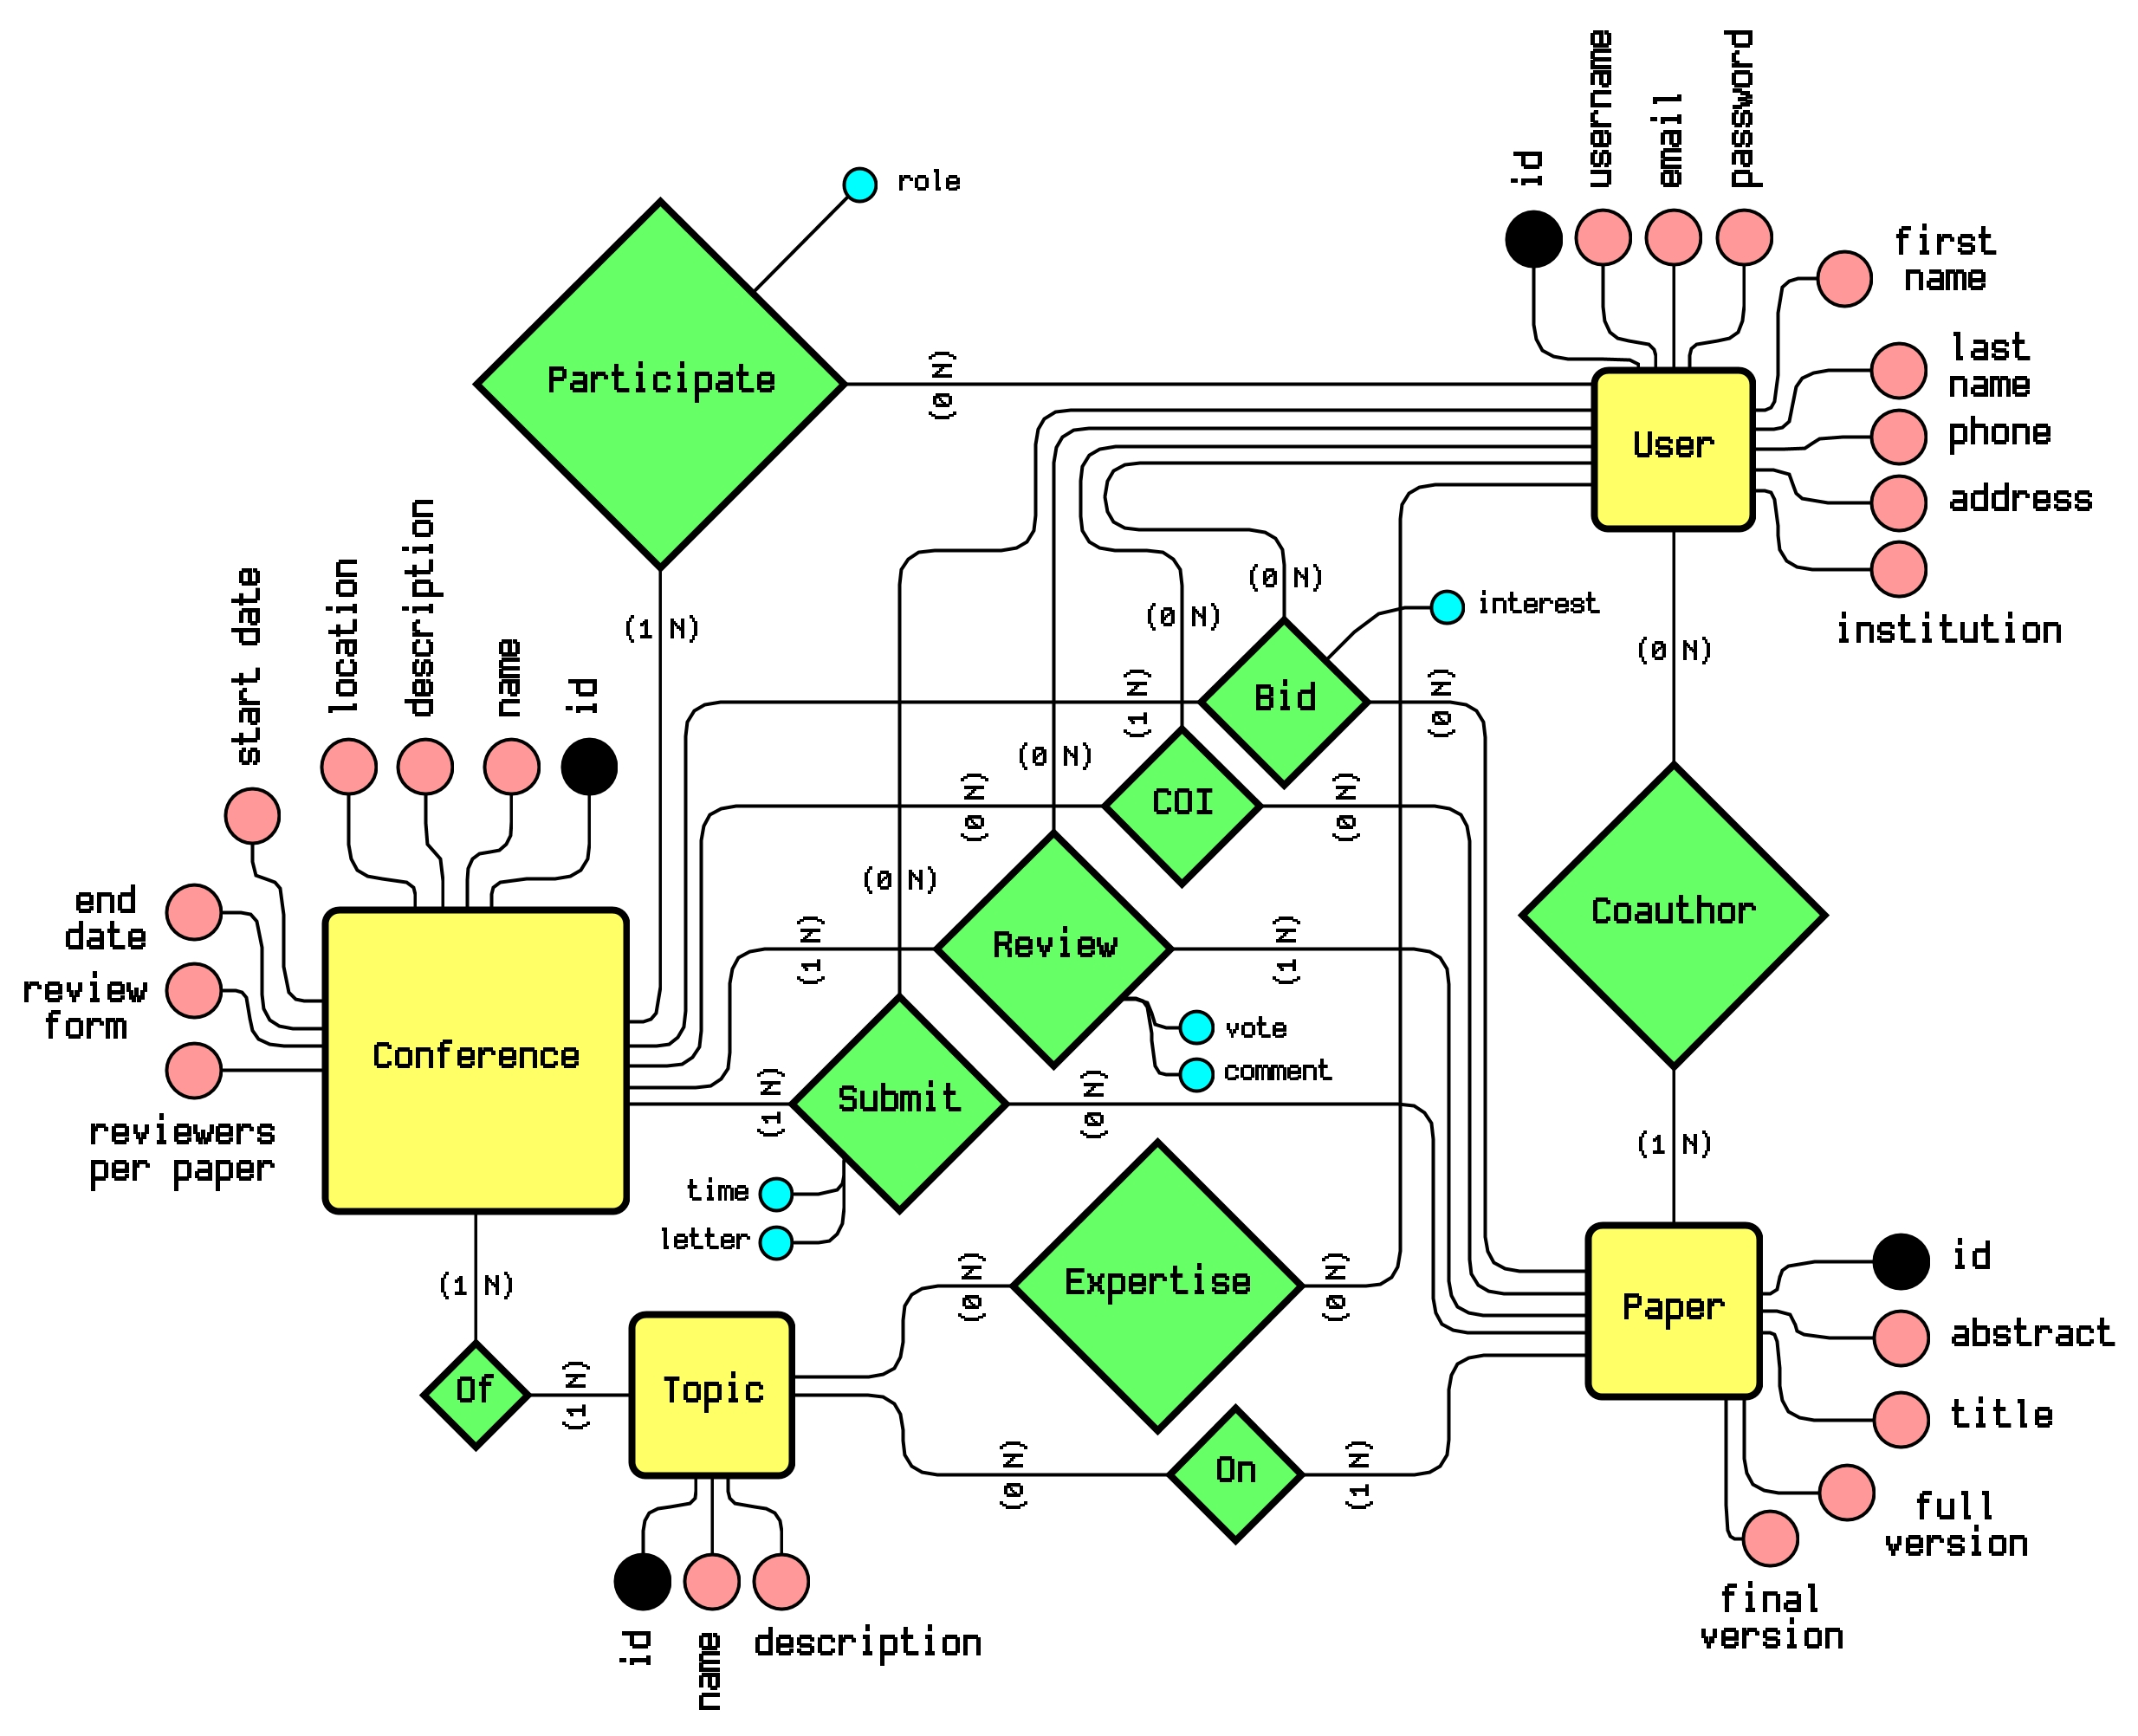
\includegraphics[angle=90,scale=0.25]{./diagram/er}
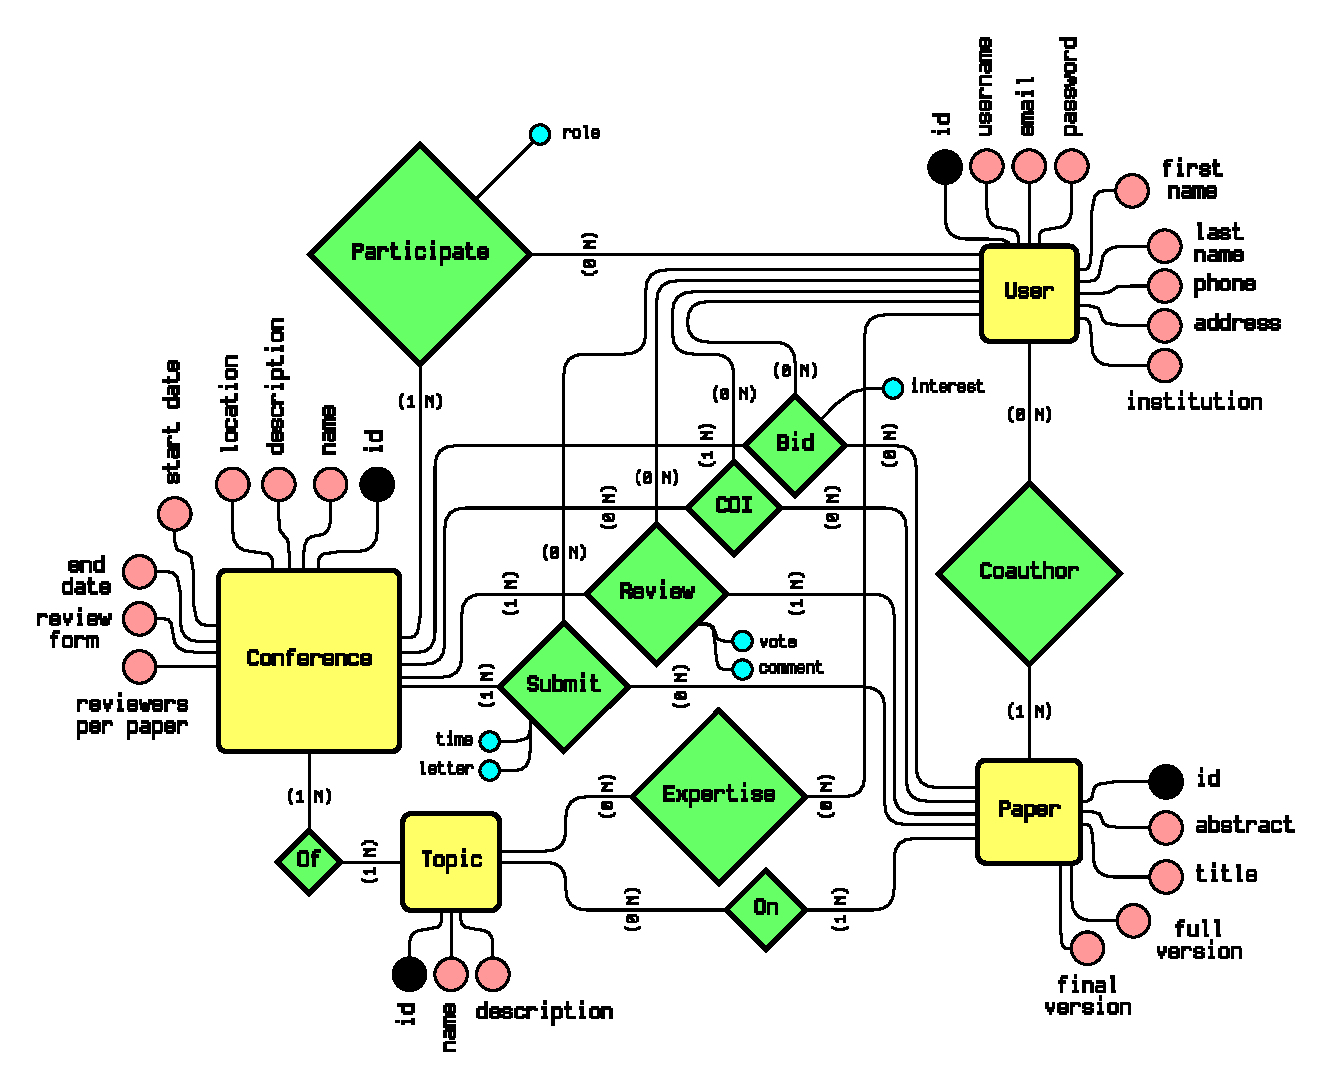
\includepdf{./diagram/er.pdf}

\part{Relational schema}

\begin{enumerate}
%USERS
\item[\textbf{Users:}](\underline{User name}, E-mail, Password, First name, Last name, Institution,\\ Address, Phone number)

%USER'S TOPICS OF EXPERTISE
\item[\textbf{User's expertise:}](\underline{User name}, \underline{Topic ID})

%USER'S BID FOR PAPER
\item[\textbf{User's bid for paper:}](\underline{User name}, \underline{Paper ID}, \underline{Conference ID},
Interest)

%USER'S CONFLICT OF INTEREST
\item[\textbf{User's COI:}](\underline{User name},
\underline{Paper ID}, \underline{Conference ID})

%USER'S REVIEW
\item[\textbf{User's review:}](\underline{User name},
\underline{Paper ID}, \underline{Conference ID}, Vote, Comment)

%USER'S SUBMISSION
\item[\textbf{User's submission:}](\underline{User name}, \underline{Paper ID}, \underline{Conference ID}, Time, Letter)

%PAPERS
\item[\textbf{Papers:}](\underline{Paper ID}, Abstract, Title, Full version, Final version)

%PAPER'S CO-AUTHORS
\item[\textbf{Paper's co-authors:}](\underline{Paper ID}, \underline{User name})

%PAPER'S TOPIC
\item[\textbf{Paper's topic:}](\underline{Paper ID}, \underline{Topic ID})

%CONFERENCES
\item[\textbf{Conferences:}](\underline{Conference ID}, Name, Description, Location, Start date, End date, Review form, Reviewers per paper)

%USERS PARTICIPATING AT CONFERENCE
\item[\textbf{Committee:}](\underline{Conference ID}, \underline{User name}, Role)

%TOPICS OF CONFERENCE
\item[\textbf{Conference's topics:}](\underline{Conference ID}, \underline{Topic ID})

%TOPICS
\item[\textbf{Topics:}](\underline{Topic ID}, Name, Description)
\end{enumerate}

\part{PostgreSQL database definition}
\end{document}%}

